\chapter{Estado da Arte}
\label{sec:2-EstadoArte}

O presente capítulo tem como objetivo a contextualização teórica do trabalho realizado. 
Primeiramente, são abordados conceitos relacionados com o projeto. De seguida, é realizado um 
levantamento das tecnologias existentes no âmbito do projeto. Por fim, são expostas algumas 
soluções semelhantes já existentes no mercado, proporcionando assim uma visão ampla do contexto em 
que o trabalho desenvolvido se insere.

\section{Sistemas Distribuídos}

Os sistemas distribuídos representam uma arquitetura de \textit{software} onde vários sistemas 
interagem entre si através de uma rede de computadores. Estes sistemas são compostos por um conjunto 
de computadores autónomos que apresentam uma visão unificada e consistente para os clientes que o 
usam. A comunicação entre os computadores é estabelecida através de mensagens, permitindo a partilha 
de recursos e a execução de tarefas em paralelo, contribuindo assim para uma maior eficiência
e escalabilidade do sistema \cite{verissimo2001distributed}.

\subsection{Arquitetura Cliente-Servidor}

A arquitetura cliente-servidor, Figura \ref{fig:client-server} é um modelo amplamente utilizado na 
computação distribuída para a troca de informações entre máquinas. Esta arquitetura envolve 
normalmente um servidor, ou um conjunto de servidores, central que fornece recursos ou serviços a 
vários clientes \cite{clientserver2019}. A comunicação entre o cliente e o servidor é realizada 
através de um protocolo de comunicação, como o HTTP ou o TCP/IP.

Além disso, a arquitetura cliente-servidor tem sido objeto de investigação em vários domínios, 
incluindo as arquiteturas de jogos \cite{clientserver2018}, a computação móvel \cite{clientserver1999},
e as infraestruturas baseadas em \textit{cloud} \cite{clientserver2012}. A escalabilidade e o 
desempenho da arquitetura têm sido investigados, com estudos centrados em mecanismos de sincronização
\cite{clientserver2004}, aplicações interativas distribuídas sem tráfego \cite{clientserver2015} e
alocação dinâmico de recursos \cite{clientserver2012}.

No contexto de arquiteturas multi servidor, a criação de servidores regionais próximos dos clientes 
tem sido explorada para resolver o problema da latência e atraso nas respostas ao cliente 
\cite{clientserver2022b}. A utilização de pseudónimos personalizados para servidores na 
\textit{cloud} foi proposta para melhorar a segurança e reduzir os custos de comunicação entre
sistemas distribuídos \cite{clientserver2017}.

\begin{figure}[H]
    \centering
    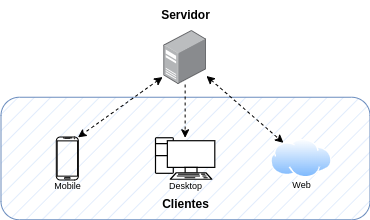
\includegraphics[width=0.5\textwidth]{media/content/estado-arte/client-server.png}
    \caption{Arquitetura Cliente-Servidor}
    \label{fig:client-server}
\end{figure}

\subsection{Arquitetura Streaming}

Os sistemas de \textit{streaming} distribuídos são cruciais para o processamento e a análise de dados 
em tempo real. O desempenho destes sistemas depende, em grande parte, da distribuição efetiva da 
carga de trabalho entre as máquinas \cite{stream2020}. Para garantir um serviço de \textit{streaming} 
eficaz e confiável, é essencial estabelecer um ambiente distribuído para o fluxo contínuo de 
informação \cite{stream2014}. A computação de \textit{streams} surgiu como uma tecnologia líder 
para analisar e gerir dados de fluxo massivo, tornando-se um modelo popular para a análise de 
fluxo de dados em tempo real \cite{stream2018} \cite{stream2018b}.

O \textit{Apache Storm}, um sistema de \textit{streaming} distribuído, foi reconhecido como um 
sistema de processamento de \textit{streams} de dados distribuídos tolerante a falhas em tempo real, 
enfatizando a importância da tolerância a falhas no processamento de \textit{streams} 
\cite{stormattwitter}. Num sistema de processamento distribuído de \textit{streams}, estes dados 
são processados em tempo real por um conjunto de operadores distribuídos por um \gls{cluster}
de servidores, o que demonstra a natureza distribuída dos sistemas de processamento do fluxos de dados.

\subsection{Problemas de consenso}

O problema do consenso em sistemas de \textit{software} distribuídos é uma questão fundamental que 
tem merecido grande atenção nos últimos anos devido à sua vasta aplicação em vários domínios, como
as redes de sensores, o controlo cooperativo de sistemas multi-agente e as redes inteligentes 
distribuídas \cite{consensus2020}. O consenso refere-se ao processo de desenvolvimento de políticas 
de controlo distribuído que permitem que um grupo de agentes seja capaz de chegar a um acordo sobre 
um determinado assunto \cite{consensus2013}. É uma questão crítica em algoritmos distribuídos e é
essencial para o funcionamento fiável de sistemas distribuídos assíncronos \cite{consesus2016} 
\cite{consensus2011}.

Além disso, o problema do consenso foi investigado no contexto de restrições e condições
específicas, como restrições de entrada e latência na comunicação, levando ao desenvolvimento de
algoritmos como o algoritmo de consenso projetado e o algoritmo de subgradiente para estimativa 
de consenso em sistemas multi-agentes com restrições convexas e atrasos de comunicação 
\cite{consensus2018}.

\section{Estratégias de implantação}

Esta secção explora algumas das abordagens de implantação e atualização de aplicações, com foco 
especial em algumas técnicas em específico como implantação \textit{canary} e \textit{rolling update}.
Ao examinar várias estratégias em detalhe, podemos capturar a essência das práticas de implantação, 
identificando os seus benefícios, desafios e áreas de aplicação mais adequadas. 

\subsection{Implantação Canary}

A técnica de implantação \textit{canary} é uma estratégia de implantação de \textit{software} que 
tem ganhado atenção na literatura nos últimos tempos. Esta técnica é brevemente introduzida no 
contexto da implantação contínua de produtos e serviços com uso intensivo de \textit{software} \cite{canary2017}. 
A estratégia de implantação \textit{canary} envolve lançar uma parte das atualizações do sistema a 
um subconjunto de utilizadores, permitindo detetar problemas antes da implantação completa.
Este processo pode ser ilustrado na Figura \ref{fig:canary-before} e na Figura \ref{fig:canary-after}. 
Esta estratégia permite uma implementação gradual e segura das alterações, minimizando o impacto 
para a maior parte do utilizadores em caso de falha. Esta estratégia é proposta para uma implantação 
bem sucedida no contexto de estratégias híbridas de implantação de \textit{software} para sistemas 
complexos \cite{canary2022}. É também importante destacar a importância das \textit{pipelines} 
automatizadas de implantação no contexto de \ac{CI} e \ac{CD}, onde o sucesso da adoção das 
alterações nas empresas depende fortemente das \textit{pipelines} de implantação 
\cite{canary2017b}. Além disso, foi proposta a utilização da implantação \textit{canary} como um 
padrão de implantação de \textit{software} para controlar a implantação de novas versões de 
\textit{software}, diminuindo o risco de falhas no processo e aumentando a fiabilidade 
\cite{canary2021}.

\begin{figure}[H]
    \centering
    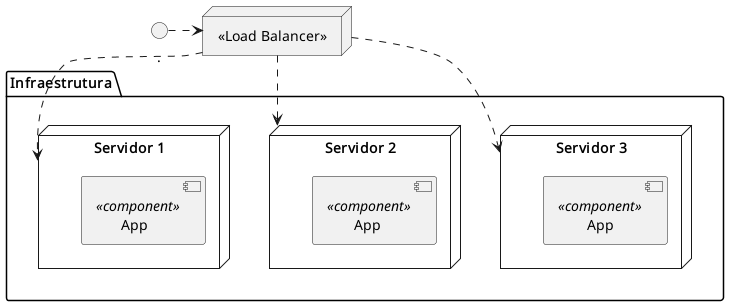
\includegraphics[width=0.4\textwidth]{media/content/estado-arte/canary-before.png}
    \caption{Estratégia de implantação \textit{canary} antes da atualização}
    \label{fig:canary-before}
\end{figure}

\begin{figure}[H]
    \centering
    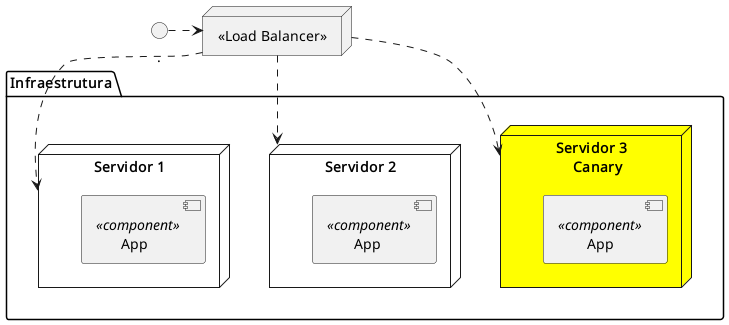
\includegraphics[width=0.4\textwidth]{media/content/estado-arte/canary-after.png}
    \caption{Estratégia de implantação \textit{canary} após a atualização}
    \label{fig:canary-after}
\end{figure}

\subsection{Rolling Update}

A estratégia de implementação de \textit{rolling update}, ou atualizações contínuas, é um aspeto 
crucial da manutenção e gestão de \textit{software}, em particular no contexto da computação em 
\textit{cloud} \cite{rolling2014}. Esta estratégia envolve atualizar gradualmente as instâncias de 
um serviço, substituindo cada instância antiga por uma nova, de forma sequencial, garantindo assim 
a disponibilidade contínua do serviço durante o processo de atualização. Nesta estratégia é destacada 
a importância da atualização contínua como uma técnica para a atualização dinâmica de \textit{software} 
que se encontra a ser utilizado ativamente por clientes \cite{rolling2014}. 

Neste tipo de abordagens é importante ter em conta a engenharia de tráfego e a necessidade de 
introduzir nós de reserva e de sentinela nas redes do sistema \cite{canary2022}, salientando a 
relevância da implementação de versões \textit{canary} como base para a estratégia de atualização 
do cliente \cite{canary2022}. A presença deste tipo de nós na rede neste tipo de estratégia é 
crucial para garantir a disponibilidade contínua do serviço durante o processo de atualização e a 
deteção de problemas antes da implantação completa.

\subsection{Blue-Green Deployment}

A implantação \textit{blue-green} é uma estratégia de implantação de \textit{software} que visa 
minimizar o tempo de indisponibilidade e os riscos associados às atualizações de \textit{software}, 
garantindo a disponibilidade e fiabilidade contínua do sistema. Esta estratégia envolve a
manutenção de dois ambientes de produção idênticos, Figura \ref{fig:blue-green-before} - o ambiente atual 
(\textit{blue}) e o novo (\textit{green}), e o encaminhamento do tráfego de utilizadores entre eles. 
Quando se pretende implantar uma nova versão do sistema, o tráfego é gradualmente transferido do 
ambiente "azul" para o ambiente "verde" como ilustrado na Figura \ref{fig:blue-green-after}, 
permitindo atualizações sem indisponibilidade e simplificando o processo de reversão das 
alterações, se necessário \cite{canary2022}.

A abordagem híbrida da implantação de software, combina a implantação \textit{canary} e a técnica 
\textit{blue-green} com a abordagem de lançamento \textit{dark} - um ambiente de intermédio, semelhante
ao de produção, que opera com dados reais - e o uso de \textit{flags} de funcionalidades, 
melhorando a estratégia global de implantação \cite{canary2022}. Esta abordagem assegura uma 
transição suave entre versões e permite a realização de testes num ambiente semelhante ao de 
produção antes da implantação para a totalidade dos utilizadores.

A técnica de implantação \textit{blue-green} baseada em descoberta de serviço em ambientes de 
\textit{cloud}, é enfatizada em ambientes modernos de computação distribuída \cite{bluegreen}. 
Desta forma, podemos concluir a importância da implantação \textit{blue-green} em sistemas baseados 
em \textit{cloud}, onde a alta disponibilidade e a interrupção mínima são cruciais.

\begin{figure}[H]
    \centering
    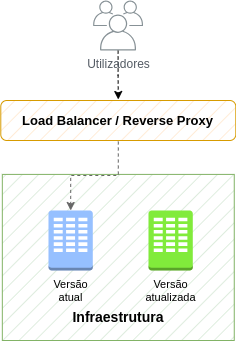
\includegraphics[width=0.3\textwidth]{media/content/estado-arte/blue-green-before.png}
    \caption{Estratégia de implantação \textit{blue-green} antes da atualização}
    \label{fig:blue-green-before}
\end{figure}

\begin{figure}[H]
    \centering
    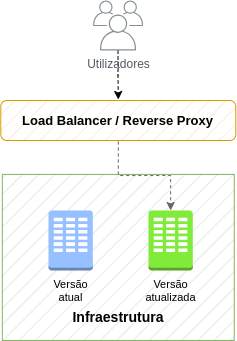
\includegraphics[width=0.3\textwidth]{media/content/estado-arte/blue-green-after.png}
    \caption{Estratégia de implantação \textit{blue-green} após a atualização}
    \label{fig:blue-green-after}
\end{figure}

\subsection{Apache Storm}

O \textit{Apache Storm} é um sistema de computação em memória distribuído e tolerante a falhas, 
concebido para processar grandes volumes de dados de alta velocidade em tempo real \cite{storm2017}. 
É um sistema centralizado e hierárquico de processamento de \textit{streams} que opera sobre o 
\textit{Nimbus} \cite{storm2015}. O \textit{Storm} permite que os operadores tenham múltiplas 
réplicas e os tuplos - a informação sobre o qual o \textit{Storm} opera - podem ser encaminhadas 
usando técnicas de agendamento como \textit{fieldsGrouping} ou \textit{partialKeyGrouping}
\cite{storm2018}. O sistema pode tirar também partido do \textit{Apache Kafka}, um serviço de 
\textit{queues} distribuído, particionado e replicado os dados de forma a integrar dados no 
\gls{cluster} de \textit{Storm} \cite{storm2018b}.

Em termos de replicação, a investigação centrou-se na implantação e replicação otimizadas do 
operador para o processamento elástico de \textit{streams} de dados distribuídos no âmbito 
da estrutura \textit{Apache Storm} \cite{storm2017b}. Os estudos integraram mecanismos ótimos de
replicação e colocação de operadores como protótipos de programadores no \textit{Apache Storm} para
melhorar o desempenho e a tolerância a falhas \cite{storm2017c}. Para além disso, o 
\textit{Apache Storm}, suporta a replicação de operadores para melhorar o desempenho quando são 
identificados pontos de acesso \cite{storm2018c}.

Relativamente às topologias - a estrutura dos serviços que operam sobre o \textit{Apache Storm} - 
é possível criar estruturas bastante complexas de processamento de fluxos. Os investigadores 
propuseram extensões ao \textit{Storm} que otimizam a paralelização dos operadores e a sua 
colocação em diferentes recursos computacionais de forma a melhorar a elasticidade e o desempenho 
do sistema \cite{storm2017d} . Além disso, o \textit{Apache Storm} tem sido utilizado em várias 
aplicações, como análise de \textit{tweets}, ambientes multi-nuvem e sistemas de análise de dados 
espaço-temporais, demonstrando sua versatilidade e ampla gama de aplicação \cite{storm2018d} 
\cite{storm2020} \cite{storm2021}.

\section{Monitorização de Sistemas}

A monitorização de sistemas de \textit{software} é uma prática essencial para garantir a saúde, 
desempenho e segurança de aplicações. Esta atividade envolve a obtenção e análise contínua de métricas, 
registos de eventos, \textit{logs} e outros dados relevantes, para avaliar o estado e o comportamento 
do sistema. Estas informações permitem tirar conclusões importantes sobre o desempenho da aplicação, 
ajudando as equipas de operações a detetar problemas, identificar tendências de comportamento, 
otimizar recursos e responder proativamente a eventos, contribuindo assim para a manutenção de 
operações eficazes.

\subsection{Métricas}

As métricas de monitorização são essenciais em projetos de \textit{software}, permitindo a descrição 
quantitativa dos projetos e a avaliação de métodos e ferramentas para aumentar a produtividade e a 
qualidade das soluções \cite{metrics2003}. Este tipo de monitorização é crucial para controlar 
projetos, produtos e processos de \textit{software} \cite{metrics2019}. As métricas permitem que os 
gestores de projetos e desenvolvedores acompanhem, e controlem, os projetos em que estão a trabalhar,
fornecendo informações sobre o estado e o progresso da solução \cite{metrics2016}. As 
métricas ajudam a estimar e a prever projetos futuros, incluindo riscos e custos 
\cite{metrics2016b}. A utilização de métricas é vital para determinar as características de 
qualidade do \textit{software} e avaliar a saúde de um projeto \cite{metrics2015}.

O \textit{Grafana} \cite{grafana}, juntamente com outras ferramentas como o \textit{Elastic Search}
\cite{elastic-search} é amplamente utilizado para visualizar dados de séries temporais e monitorizar
a evolução de questões de dívida técnica em projetos de \textit{software} \cite{metrics2019b}. O 
\textit{Grafana} é também utilizado para obter, armazenar e visualizar metadados produzidos por 
sistemas de gestão de dados e fluxo de trabalho, demonstrando a sua importância na monitorização 
de projetos \cite{metrics2021}. O \textit{Grafana} serve como uma ferramenta de visualização para 
processar pontos de dados brutos e interfaces de monitorização, destacando sua versatilidade na 
monitorização de projetos de \textit{software} \cite{metrics2022}.

\subsection{Registo de eventos}

O registo de eventos desempenha um papel crucial na engenharia de \textit{software} uma vez que 
fornece uma noção das atividades e dos eventos que ocorrem no sistema \cite{logs2022}. A profundidade 
do conhecimento disponível nos \textit{logs} levou ao desenvolvimento de plataformas comerciais de 
análise deste tipo de eventos, como o \textit{Splunk} \cite{splunk}, que são essenciais para 
analisar e compreender os dados de \textit{logs} \cite{logs2021}. No entanto, existem desafios nos 
registos de eventos durante o desenvolvimento de projetos de \textit{software}, particularmente em 
projetos \textit{open source}, o que leva a uma redução na rastreabilidade dos defeitos e à
deteção de \textit{bugs} de \textit{software} \cite{logs2018}. Os \textit{logs} servem diferentes 
propósitos, como deteção de anomalias, diagnóstico de problemas, verificação de programas, análise 
de uso e monitorização  de segurança, destacando assim a sua importância em sistemas de
\textit{software} robustos e seguros \cite{logs2019}.

